% !TEX root = main.tex

\chapter{実験結果}

本章では3.1節ではブロードコンタクトレーザー、3.2節ではリッジ導波路型レーザーへの電流注入実験についての実験結果を報告する。
\section{ブロードコンタクトレーザー試料に関する測定結果}%=====================================
ブロードコンタクトレーザーへ定常電流を流してILカーブを得る実験を行った。様々な共振器長、電極パッド幅の試料に対して実験を行うことでウエハの基本的な物性パラメータを見積もることが目的である。

発振閾値電流を測定することに加えて、発振時の印可電流の増分に対する光出力の増大から発光量子効率(微分外部量子効率)を見積もることが目的である。
また発振閾値電流密度を算出するためにデバイス内の電流の広がりを見積もった。
3周期ウエハと10周期ウエハごとに節を分けている。
\subsection{3周期}%===============================
3周期量子井戸ブロードコンタクトレーザーの結果を示す。図\ref{fig:fig_3_1_3QW_broacdcontact_IL}(a)縦軸に発光強度(片方の端面)、横軸に電流をとったILカーブの結果である。また\ref{fig:fig_3_1_3QW_broacdcontact_IL}(b)は縦軸に試料にかかっている電圧、横軸に電流をとったIVカーブの結果である。共振器長LがL=500,1000,2000umの結果をプロットした。代表としてパッド幅w=50umの結果をプロットした。測定条件は1usパルスを2ms繰り返し周期である。デューティー比は1:2000である。

(a)を見ると各デバイスにおいて光出力強度が電流値を上げてくと増加していき、ある電流値を超えると発振が始まり発光強度が急激に増加することがわかる。その電流値を発振している時のILカーブを直線フィッティングすることで求めた。フィッティング直線のx切片を発振閾値電流$I_{\rm{th}}$とした。またフィッティング直線の傾きを発振時のスロープ効率$\Delta P/\Delta I$とした。
ここで表とか作った方がわかりやすいか?

(b)を見ると各デバイスにおいて電流が流れ始めるのが1V付近からであることが見て取れる。また共振器長Lが長いほど同じ電流に対する電圧が低い。これは電流が流れる面積が共振器長Lに比例して大きくなるためデバイスの抵抗値が小さくなっているためである。
\begin{figure}[h]
	\centering
	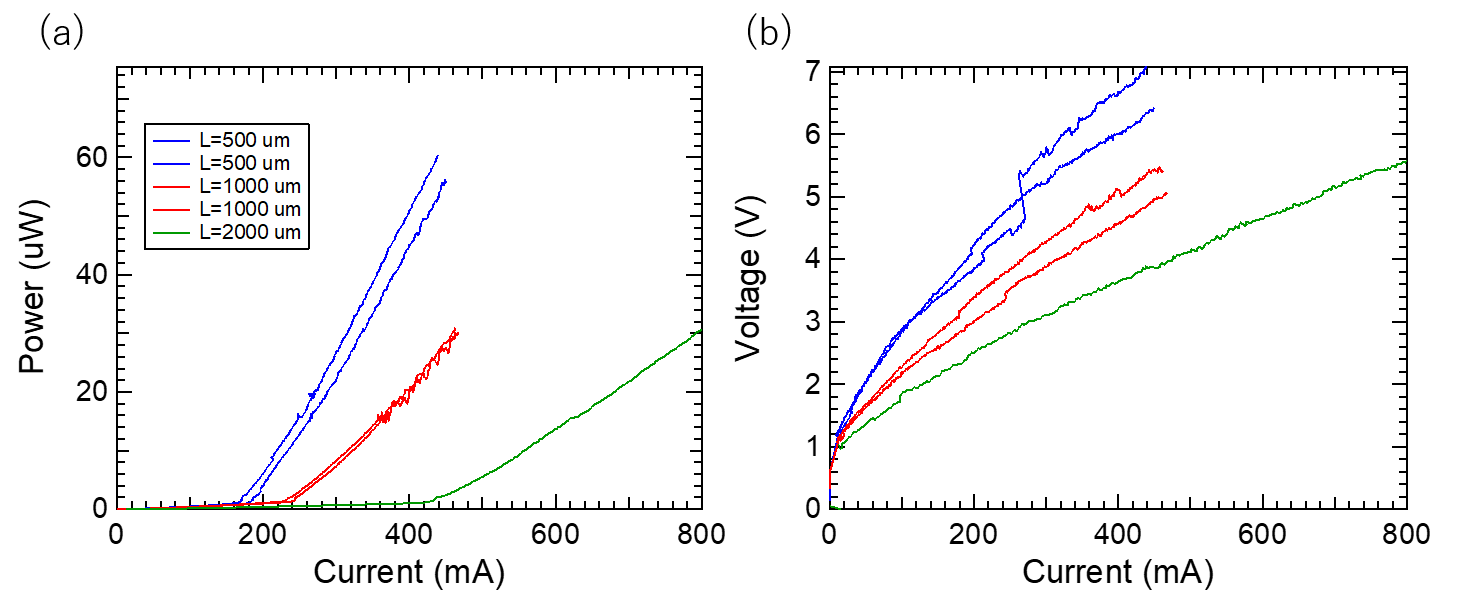
\includegraphics[width=15cm]{figure/fig_3_1_3QW_broadcontact_IL.png}
		\caption{3MQWのILカーブとIVカーブ}
		\label{fig:fig_3_1_3QW_broacdcontact_IL}
\end{figure}

\clearpage
次に様々なパッド幅に対して見積もった発振閾値電流$I_{\rm{th}}$の結果を図\ref{fig:fig_3_1_3QW_broadcontact_Ith}(a)に示す。発振閾値電流$I_{\rm{th}}$、横軸が電極パッド幅wである。(b)は発振時の発光効率である。先のフィッティング直線の傾きにデューティー比をかけ、さらに両端面からの発光の分で2倍したものをプロットした。

図\ref{fig:fig_3_1_3QW_broadcontact_Ith}(a)を見ると、パッド幅wが50umより大きい領域では閾値電流$I_{\rm{th}}$はパッド幅wに対して線形に増加していることがわかる。一方パッド幅wが小さい領域では線形に変化していない。

この原因は電流がパッド幅wに対して無視できないほど広がってしまっているためだと考えられる。このことについて3.1.3節で述べる。

図\ref{fig:fig_3_1_3QW_broadcontact_Ith}(b)を見るとそれぞれの共振器長で概ね横ばいの値を持っている。

\begin{figure}[hb]
	\centering
	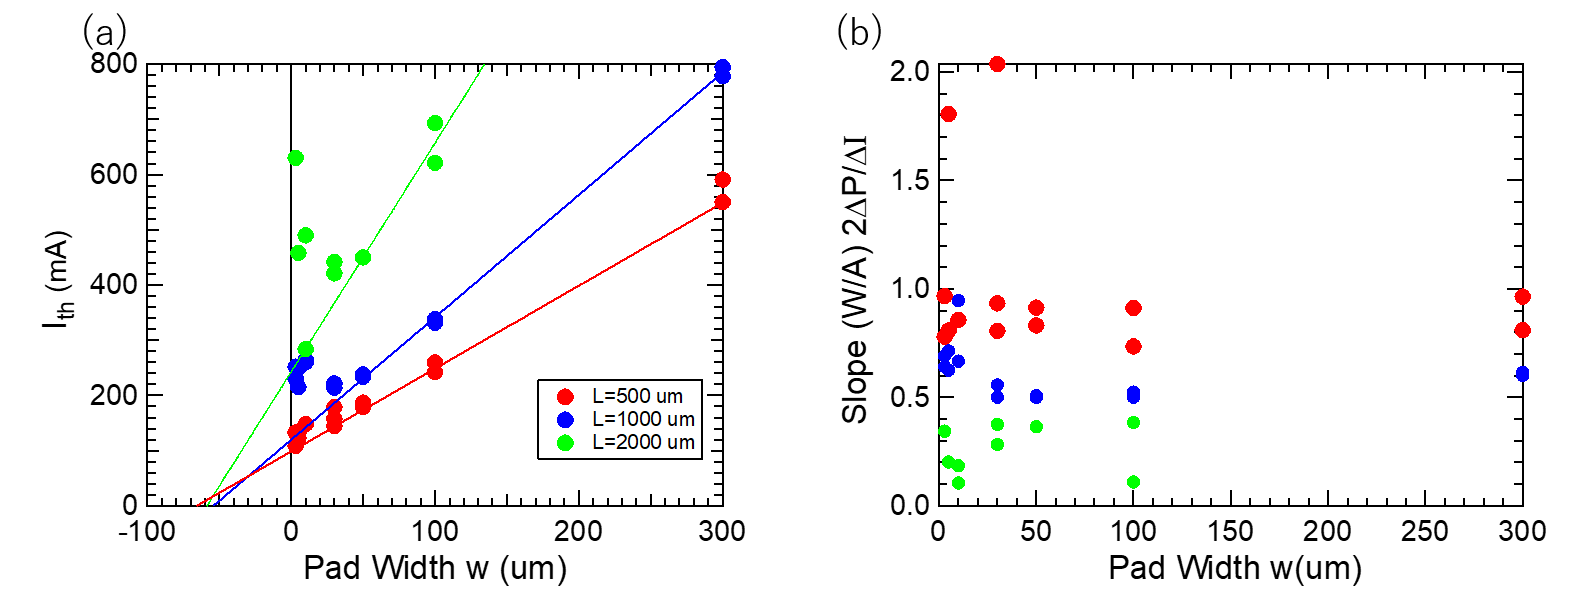
\includegraphics[width=15cm]{figure/fig_3_1_3QW_broadcontact_Ith.png}
		\caption{3MQWの閾値電流と発光効率}
		\label{fig:fig_3_1_3QW_broadcontact_Ith}
\end{figure}
\clearpage
\subsection{10QW}%===============================
次に10周期量子井戸ブロードコンタクトレーザーについての結果を示す。図\ref{fig:fig_3_1_10QW_broadcontact_IL}に(a)ILカーブおよび(b)IVカーブを示す。w=50umを代表としてプロットした。色分けは共振器長を表す。駆動条件は2usパルスを2ms繰り返し周期で印可した。デューティー比は1:1000である。
\begin{figure}[h]
	\centering
	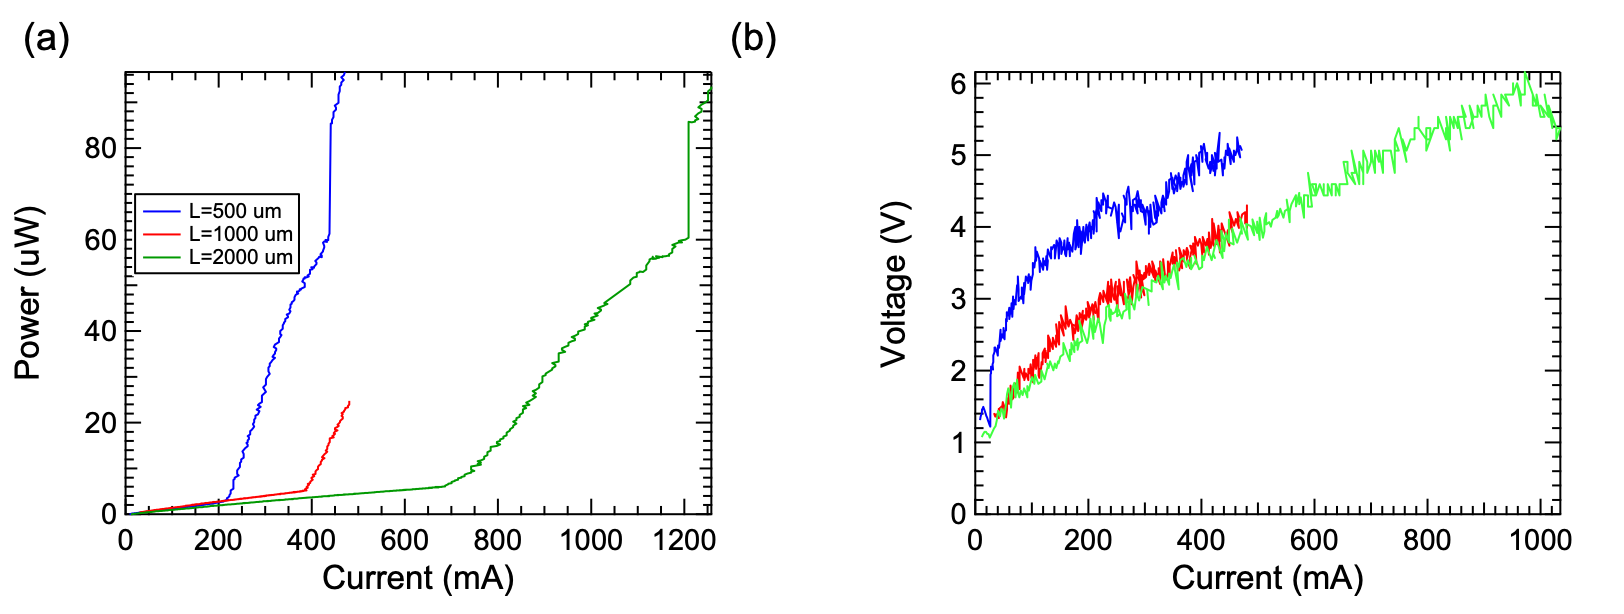
\includegraphics[width=15cm]{figure/fig_3_1_10QW_broadcontact_IL.png}
		\caption{10MQWのIL結果}
		\label{fig:fig_3_1_10QW_broadcontact_IL}
\end{figure}
次に\ref{fig:fig_3_1_3QW_broadcontact_Ith} (a)に\ref{fig:fig_3_1_10QW_broadcontact_IL} (a)のILカーブの発振時の直線フィッティング結果から閾値電流$I_{\rm{th}}$および(b)スロープ効率$\Delta P/\Delta I$をプロットした。傾きはデューティー比1:1000と両端面からの発光を換算していることに注意されたい。
\begin{figure}[h]
	\centering
	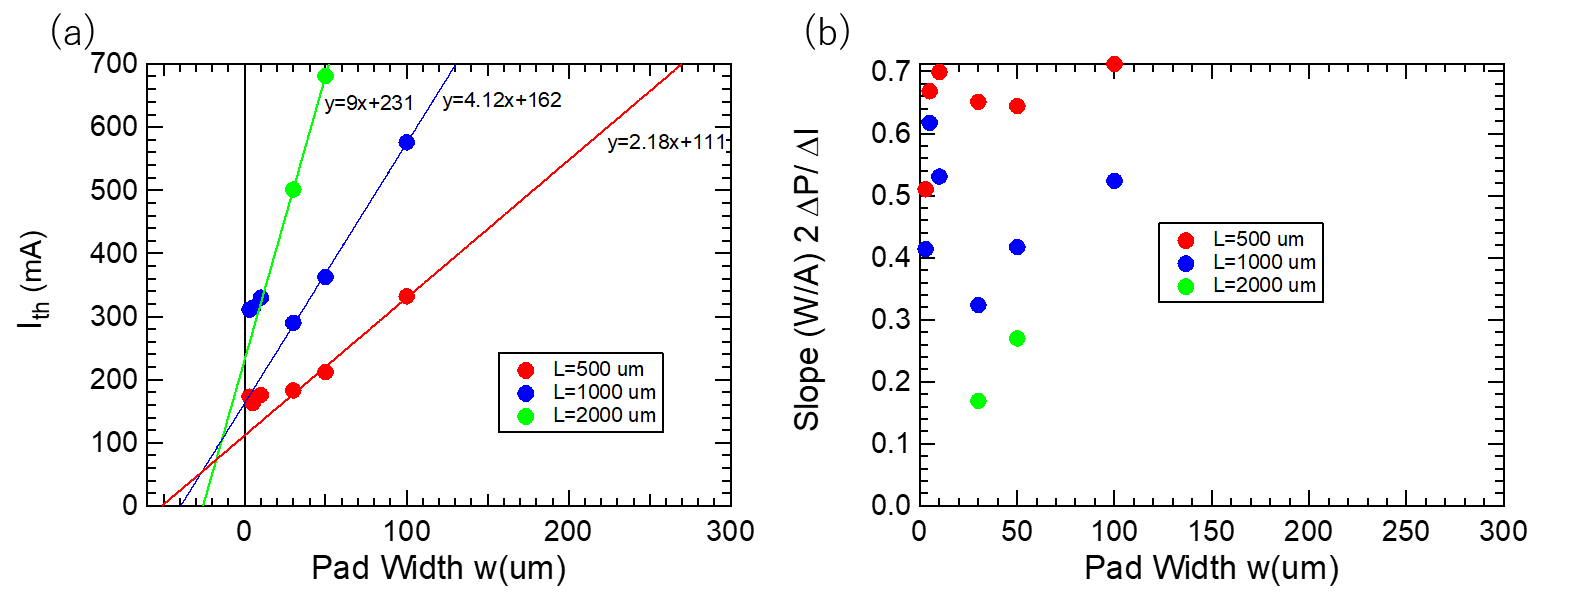
\includegraphics[width=15cm]{figure/fig_3_1_10QW_broadcontact_Ith.png}
		\caption{10MQWのIL結果}
		\label{fig:fig_3_1_10QW_broadcontact_Ith}
\end{figure}
\subsection{電流広がりに関する考察}%==================
3.1.1節と3.1.2節でILカーブから閾値電流を見積もった。この値から閾値電流密度$J_{\rm{th}}$を求めることが大切である。
レーザーの基本的な特性を知る上で閾値電流密度が大切なパラメータであるからである。発振閾値電流$I_{\rm{th}}$を電流が流れた面積で割れることで閾値電流密度$J_{\rm{th}}$が求まる。\\
 本体閾値電流電流は電流を流す面積に比例して大きくなる。面積とは電極パッド幅wと共振器長Lの積で表される。しかし図\ref{fig:fig_3_1_3QW_broacdcontact_IL} (a)や\ref{fig:fig_3_1_10QW_broadcontact_IL}(a) を見るとそうなっていない。そこで発振閾値電流$I_{\rm{th}}$が線形に増加する領域をフィッティングした直線のx切片を含めたパッド幅を有効的なパッド幅と考えて閾値電流密度を算出した。まずは有効パッド幅を見積もった。フィッティング関数のx切片の絶対値が実質的なパッド幅の増分w'である。その値を表に示した。
\begin{table}[hbtp]
  \caption{3QWブロードコンタクトレーザーの電流広がり}
  \label{table:table_3QW_broadcontact_w_eff}
  \centering
  \begin{tabular}{lcr}
    \hline
    共振器長L (um)  & パッド幅の増分(電流の広がり) w' (um)   \\
    \hline \hline
     500 & 65.8  \\
    1000  & 54.1 \\
    2000  & 58.7 \\ 
    \hline
  \end{tabular}
\end{table}

\begin{table}[hbtp]
  \caption{10QWブロードコンタクトレーザーの電流広がり}
  \label{table:table_10QW_broadcontact_w_eff}
  \centering
  \begin{tabular}{lcr}
    \hline
    共振器長L (um)  & パッド幅の増分(電流の広がり) w' (um)   \\
    \hline \hline
     500 & 51.1  \\
    1000  & 39.5 \\
    2000  & 25.7 \\ 
    \hline
  \end{tabular}
\end{table}
この表の値w'と閾値電流$I_{\rm{th}}$(mA)から式(\ref{eq:Jth})の関係を用いて閾値電流密度$J_{\rm{th}} \rm{(kA/cm^2)}$を算出した。
\begin{eqnarray}
J_{\rm{th}}=\dfrac{I_{\rm{th}}}{(w+w')L}
\label{eq:Jth}
\end{eqnarray}

その結果を示す。図\ref{fig:fig_3_1_3QW_broadcontact_Ith}に3周期の結果、\ref{fig:fig_3_1_10QW_broadcontact_Ith}に10周期の結果をプロットした。
\begin{figure}[h]
	\centering
	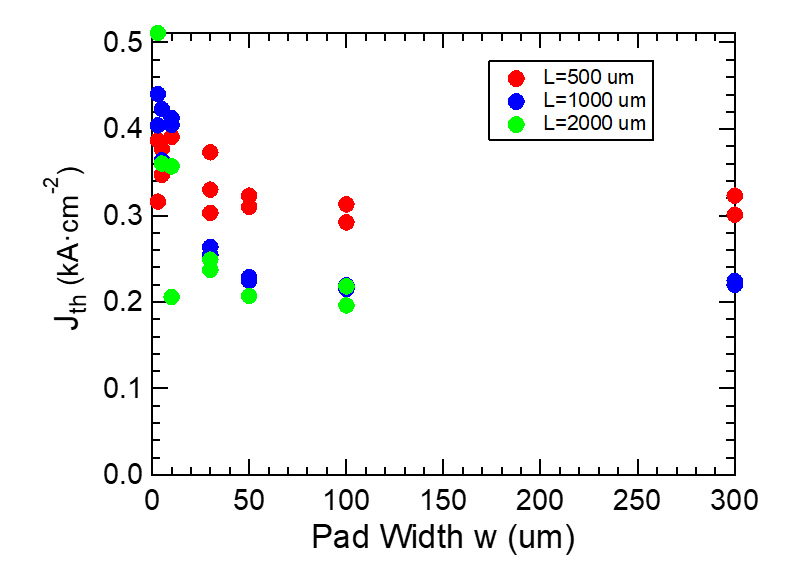
\includegraphics[width=10cm]{figure/fig_3_1_3QW_broadcontact_Jth.png}
		\caption{3MQWの閾値電流密度}
		\label{fig:fig_3_1_3QW_broadcontact_Ith}
\end{figure}

\begin{figure}[h]
	\centering
	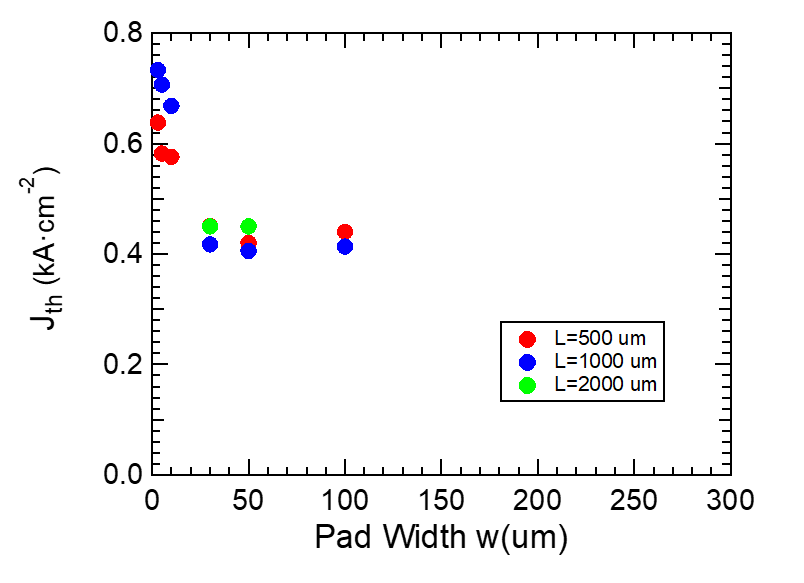
\includegraphics[width=10cm]{figure/fig_3_1_10QW_broadcontact_Jth.png}
		\caption{10MQWの閾値電流密度}
		\label{fig:fig_3_1_10QW_broadcontact_Ith}
\end{figure}
\clearpage
\subsection{外部量子効率、内部量子効率と吸収係数の計算}%=============
次にILカーブの発振時の傾きに相当するスロープ効率$\Delta P/\Delta I$から試料の内部量子効率および吸収係数を算出した。まずはスロープ効率$\Delta P/\Delta I \rm{(W/A)}$から外部微分量子効率$\eta_{\rm{d}}$を算出した。式({\ref{eq:eta_d})の関係を用いた。
\begin{eqnarray}
\eta_{\rm{d}}=\dfrac{e}{h\nu}2\dfrac{\Delta P}{\Delta I} 
\label{eq:eta_d}
\end{eqnarray}
eは電気素量、hはプランク定数、$\nu$は発振周波数であり、1050nmとした。$\eta_{\rm{d}}$はキャリアの注入数に対する取り出せる光子の数の割合である。結果を図\ref{fig:fig_3_1_3QW_broadcontact_id}に示す。縦軸を$\eta_{\rm{d}}$横軸をパッド幅wとしてプロットした。色分けが共振器長の違いを表している。L=500umでは0.7程度、L=1000umでは0.4程度、L=400umでは0.3程度の値を持っている。
\begin{figure}[h]
	\centering
	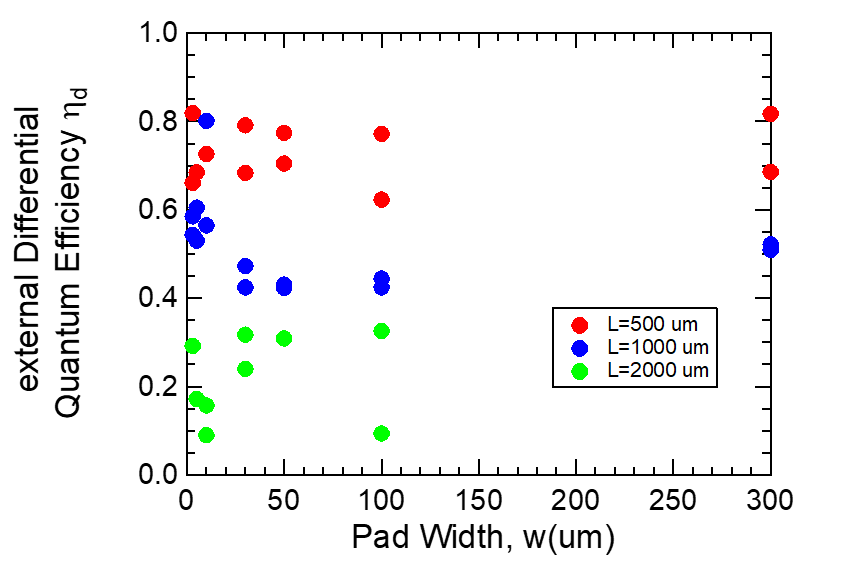
\includegraphics[width=10cm]{figure/fig_3_1_3QW_broadcontact_id.png}
	\caption{3QW外部量子効率}
	\label{fig:fig_3_1_3QW_broadcontact_id}
\end{figure}
$\eta_{\rm{d}}$は共振器長Lを用いて式(\ref{eq:eta_inverse})と書き表される。
\begin{eqnarray}
\dfrac{1}{\eta_{\rm{d}}}=\dfrac{\alpha_{\rm{int}}}{\rm{ln}(1/R)\eta_{int}}+\dfrac{1}{\eta_{\rm{int}}}
\label{eq:eta_inverse}
\end{eqnarray}
$\alpha$は共振器内の内部損失、Rは共振器のミラーロス、$\eta_{\rm{int}}$は内部微分量子効率である。Rは半導体デバイスの屈折率と空気の屈折率の差から0.32と仮定できる。見積もった$\eta_{\rm{d}}$の逆数を共振器長に対してプロットし直線フィッティングを行なった。これを図\ref{fig:fig_3_1_3QW_broadcontact_id_inverse}に示す。例としてパッド幅w=100umの結果を示す。式\ref{eq:eta_inverse}よりこのフィッティング直線のy切片から内部量子効率$\eta_{\rm{int}}$を見積もると$\eta_{\rm{int}}$=0.96と計算できる。また、直線の傾きから内部ロス$\alpha_{\rm{int}}$を見積もると$\alpha_{\rm{int}}$=11.8 (/cm)と計算できる。
\begin{figure}[h]
	\centering
	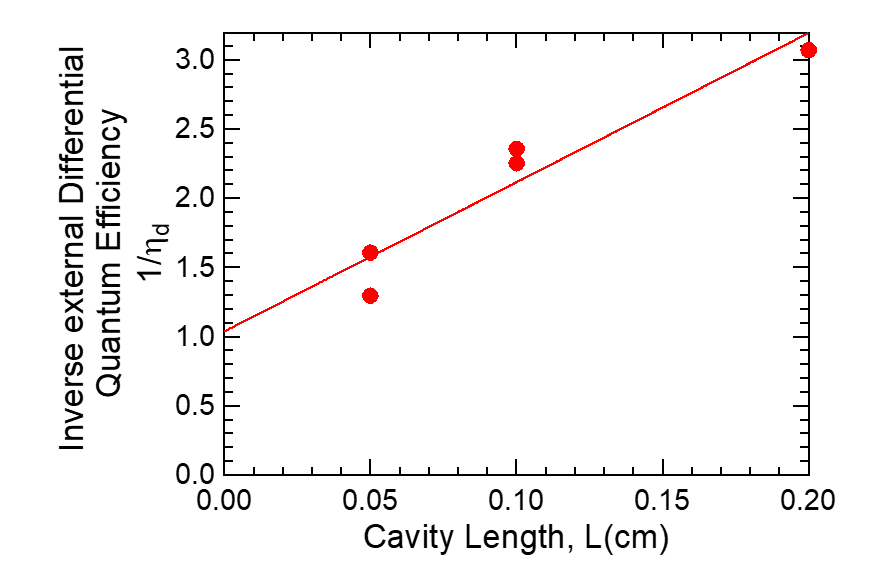
\includegraphics[width=10cm]{figure/fig_3_1_3QW_broadcontact_id_inverse.png}
	\caption{3QW外部量子効率の逆数}
	\label{fig:fig_3_1_3QW_broadcontact_id_inverse}
\end{figure}
\clearpage
同様の解析を10QWについても行った。こちらはw=50um の結果を示している。10周期に関しては$\eta_{\rm{int}}$=0.94,$\alpha_{\rm{int}}$=18.0 (/cm)となった。
\begin{figure}[h]
	\centering
	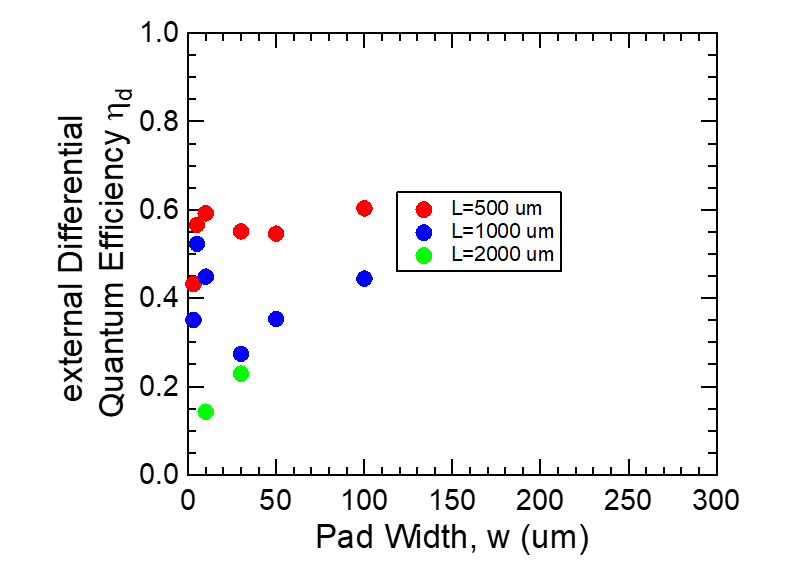
\includegraphics[width=10cm]{figure/fig_3_1_10QW_broadcontact_id.png}
	\caption{10QW外部量子効率}
	\label{fig:fig_3_1_10QW_broadcontact_id}
\end{figure}

\begin{figure}[h]
	\centering
	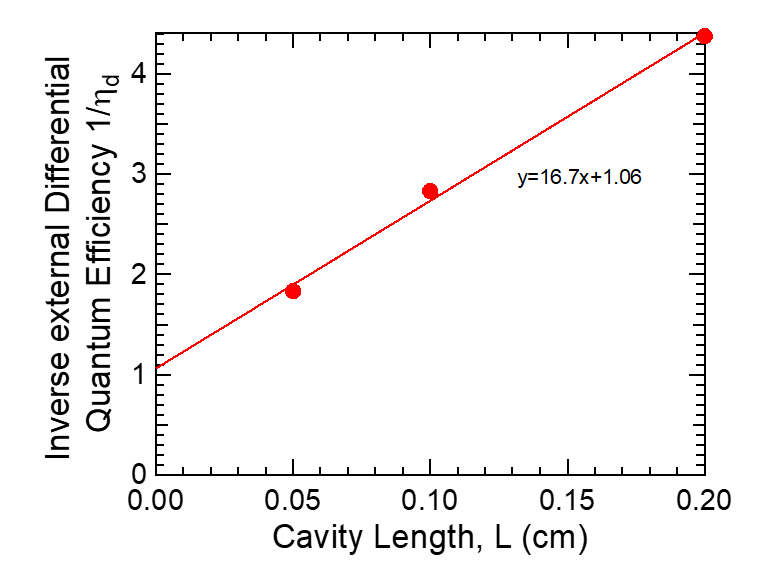
\includegraphics[width=10cm]{figure/fig_3_1_10QW_broadcontact_id_inverse.png}
	\caption{10QW外部量子効率の逆数}
	\label{fig:fig_3_1_10QW_broadcontact_id_inverse}
\end{figure}


\clearpage
\section{リッジ導波路型レーザーに関する実験結果}%===================
\subsection{定常電流の結果}
作製したリッジ導波路型レーザーのついて定常電流を流し、発光測定を行った。その結果を示す。2マイクロ秒パルスを2ミリ秒周期で注入した。デューティー比は1:1000である。
まずは3周期の結果
\begin{figure}[h]
	\centering
	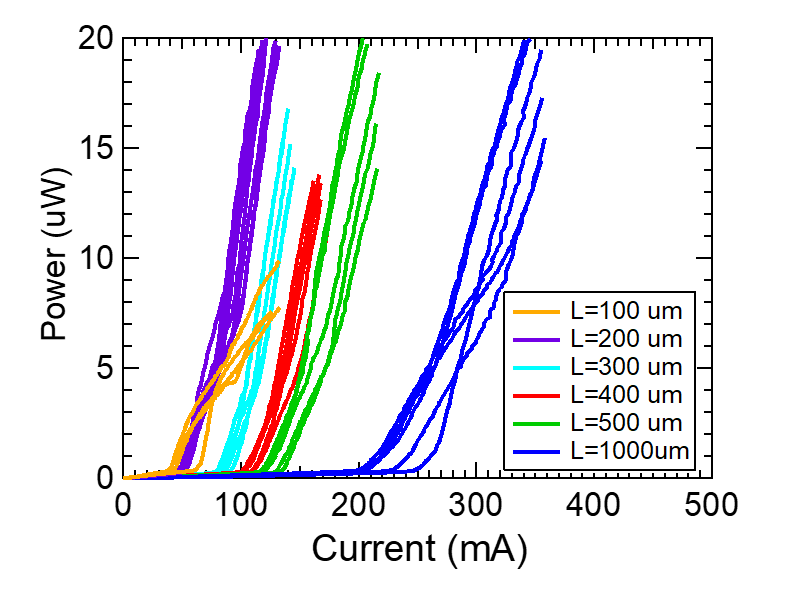
\includegraphics[width=15cm]{figure/fig_3_2_3QW_ridge_IL.png}
		\caption{3周期 リッジ導波路型レーザーのILカーブおよびIVカーブ}
		\label{fig:fig_3_2_3QW_ridge_IL}
\end{figure}
\begin{figure}[h]
	\centering
	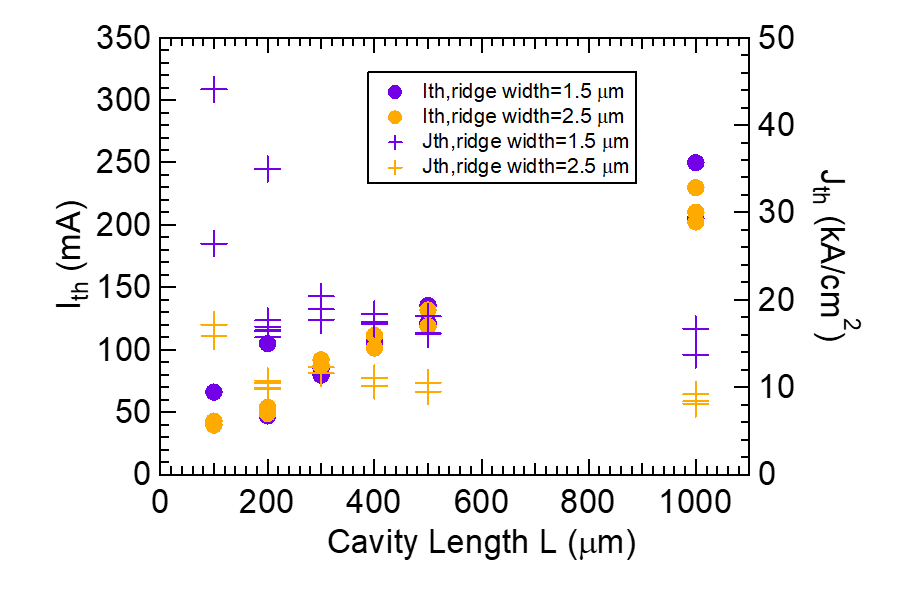
\includegraphics[width=15cm]{figure/fig_3_2_3QW_ridge_Ith.png}
		\caption{3周期 リッジ導波路型レーザーの閾値電流}
		\label{fig:fig_3_2_3QW_ridge_Ith}
\end{figure}

\begin{figure}[h]
	\centering
	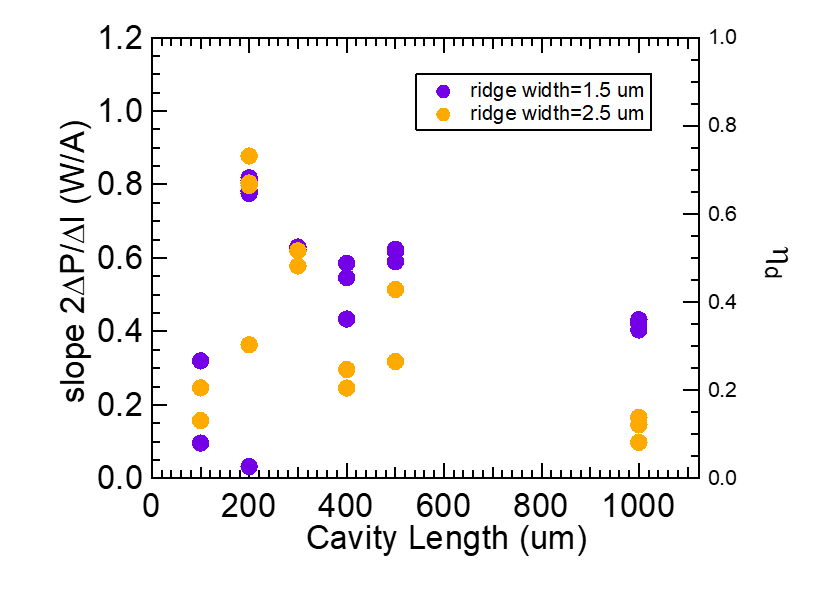
\includegraphics[width=15cm]{figure/fig_3_2_3QW_ridge_slope.png}
		\caption{3周期 リッジ導波路型レーザーのスロープ効率}
		\label{fig:fig_3_2_3QW_ridge_slope}
\end{figure}
\clearpage
次に10周期の結果を示す。
\begin{figure}[h]
	\centering
	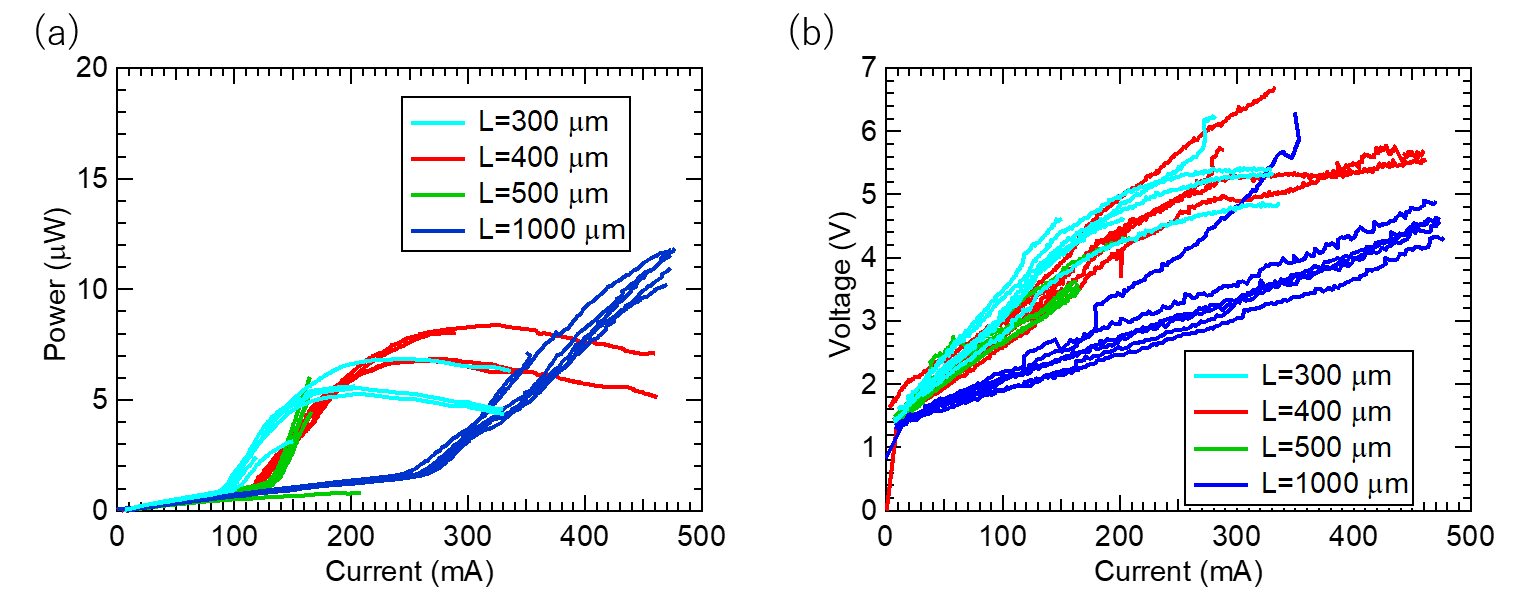
\includegraphics[width=15cm]{figure/fig_3_2_10QW_ridge_IL.png}
		\caption{10周期 リッジ導波路型レーザーのILカーブおよびIVカーブ}
		\label{fig:fig_3_2_10QW_ridge_IL}
\end{figure}
ILカーブから閾値電流と発進時の傾きを出した。それを示す。
\begin{figure}[h]
	\centering
	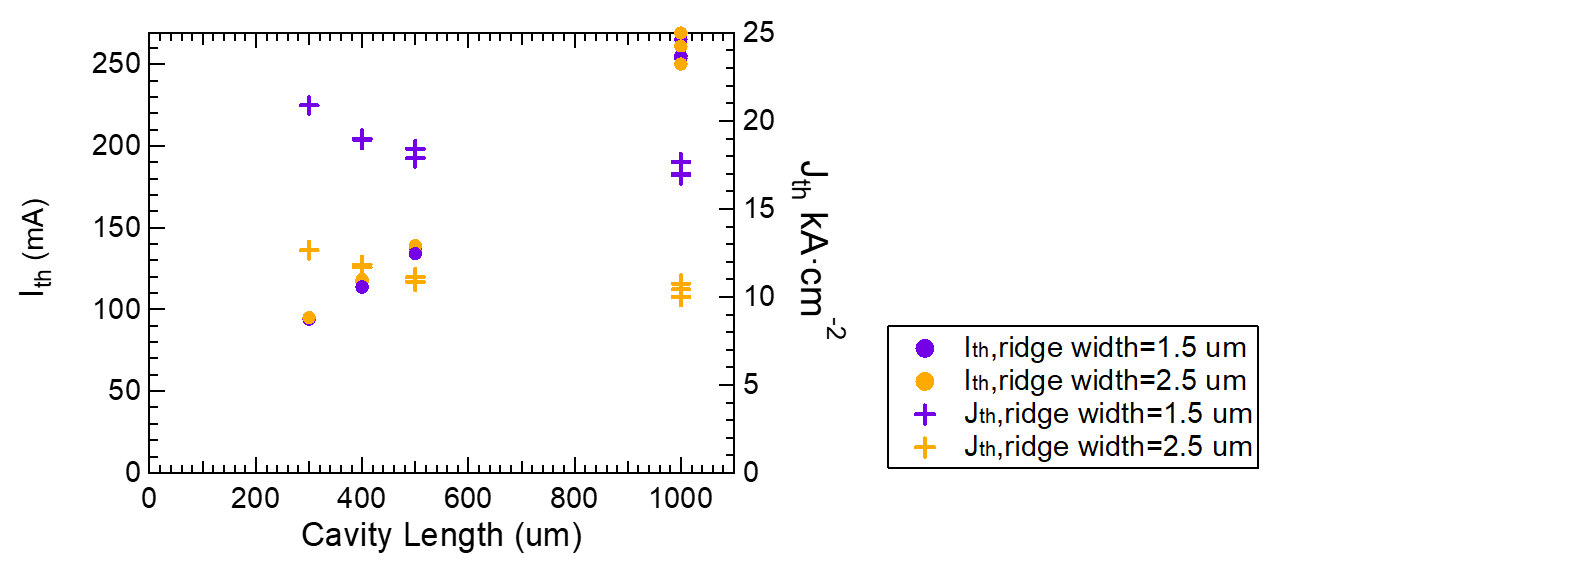
\includegraphics[width=15cm]{figure/fig_3_2_10QW_ridge_Ith.png}
		\caption{10周期 リッジ導波路型レーザーの閾値電流と閾値電流密度}
		\label{fig:fig_3_2_10QW_ridge_Ith}
\end{figure}
\begin{figure}[h]
	\centering
	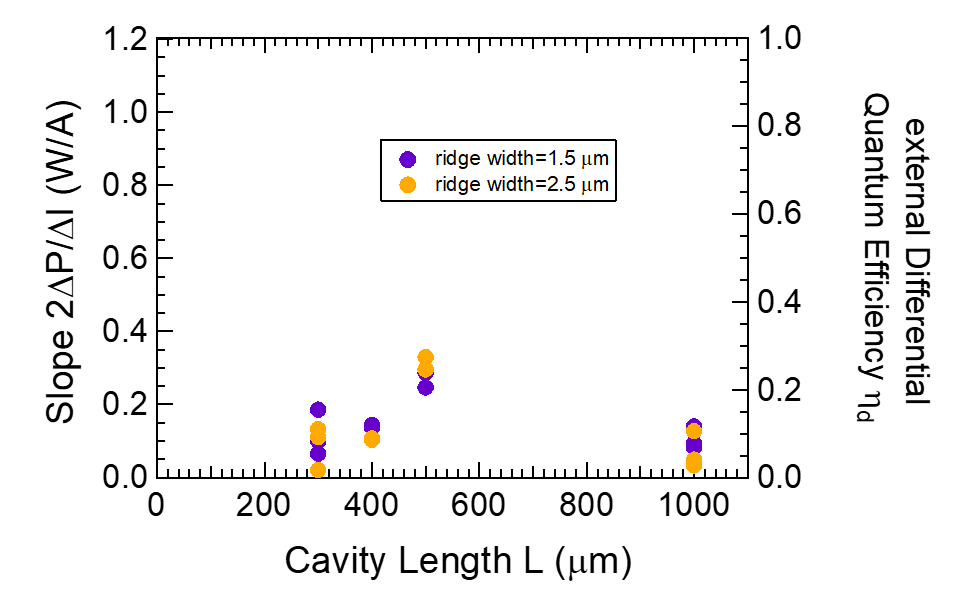
\includegraphics[width=15cm]{figure/fig_3_2_10QW_ridge_slope.png}
		\caption{10周期 リッジ導波路型レーザーのスロープ効率}
		\label{fig:fig_3_2_10QW_ridge_slope}
\end{figure}
\clearpage
\subsection{短パルス電流注入の結果}
リッジ導波路型レーザーに関して電流注入利得スイッチング実験を行った。そのILと時間波形を示す。
\subsection{IL}
10周期と3周期一個づつ
\begin{figure}[h]
	\centering
	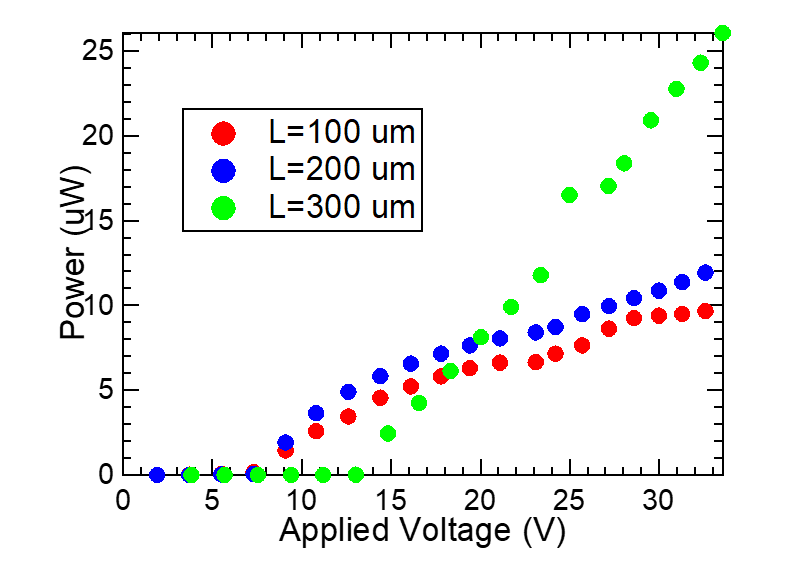
\includegraphics[width=15cm]{figure/fig_3_2_3QW_ridge_GS_power.png}
		\caption{3MQW 短パルス駆動時のILカーブ}
		\label{fig:fig_3_2_3QW_ridge_GS_power}
\end{figure}

\begin{figure}[h]
	\centering
	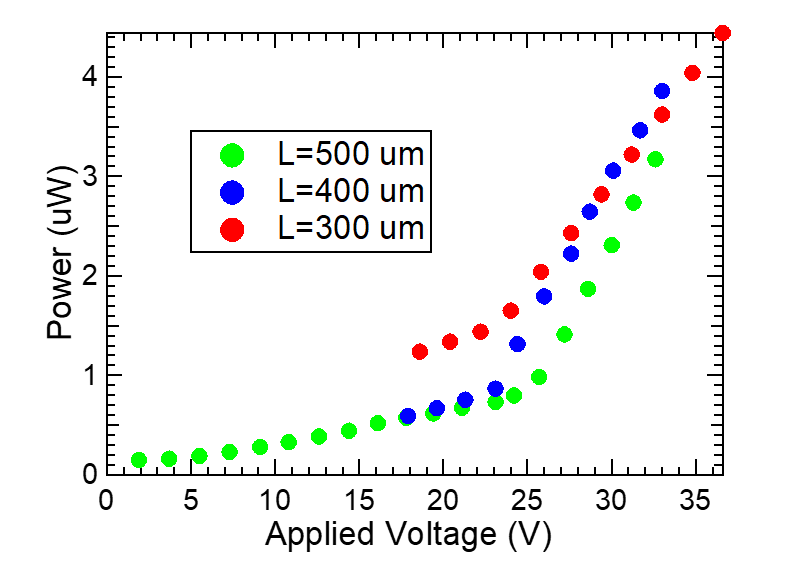
\includegraphics[width=15cm]{figure/fig_3_2_10QW_ridge_GS_power.png}
		\caption{10MQW 短パルス駆動時のILカーブ}
		\label{fig:fig_3_2_10QW_ridge_GS_power}
\end{figure}
\clearpage
\subsection{3QW試料の利得スイッチング動作}%===============================
時間波形を示す。図\ref{fig:fig_3_2_3QW_ridge_L100_GS}(a)に3周期量子井戸レーザーの励起強度を変えたときの時間波形を示す。図\ref{fig:fig_3_2_3QW_ridge_L100_GS}(b)には強度を規格化したプロットをしめす。これらを見ると励起強度を大きくするに従ってピーク強度が高くなっていき、また立ち上がりが早くなっていることがわかる。
\begin{figure}[h]
	\centering
	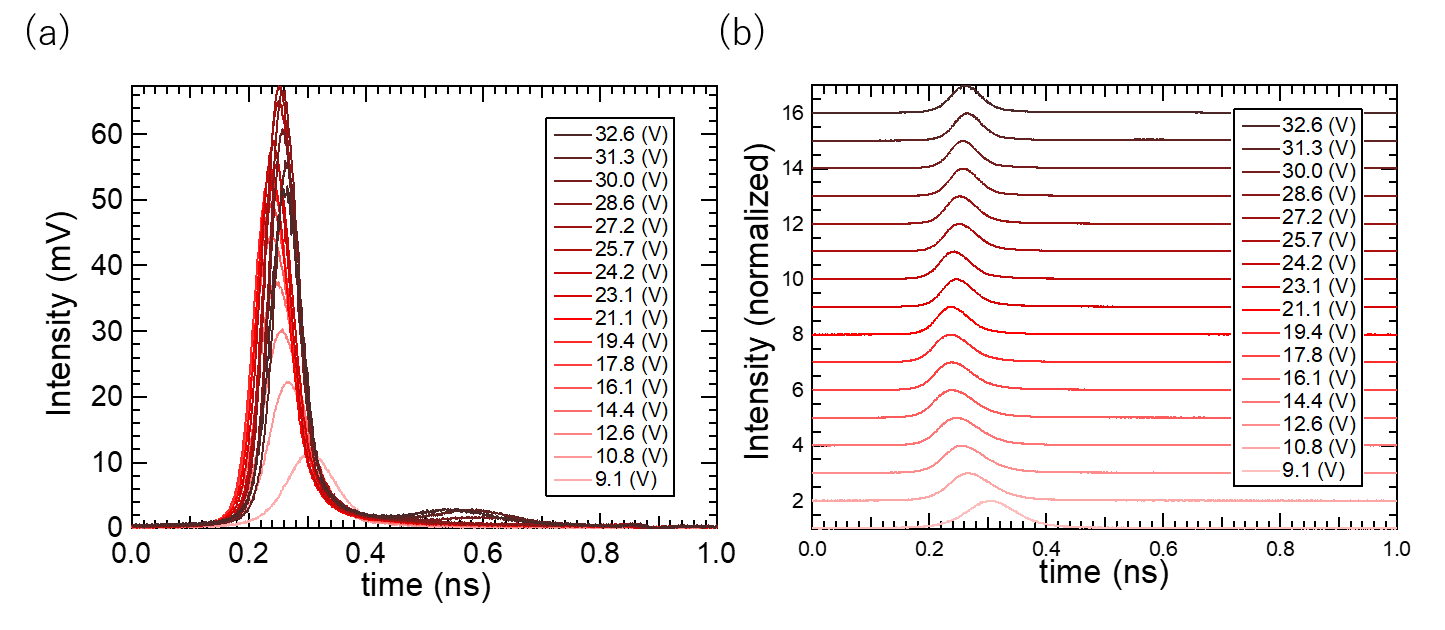
\includegraphics[width=15cm]{figure/fig_3_2_3QW_ridge_L100_GS.png}
		\caption{3MQW L=100um の利得スイッチング光パルスの時間波形}
		\label{fig:fig_3_2_3QW_ridge_L100_GS}
\end{figure}

\begin{figure}[h]
	\centering
	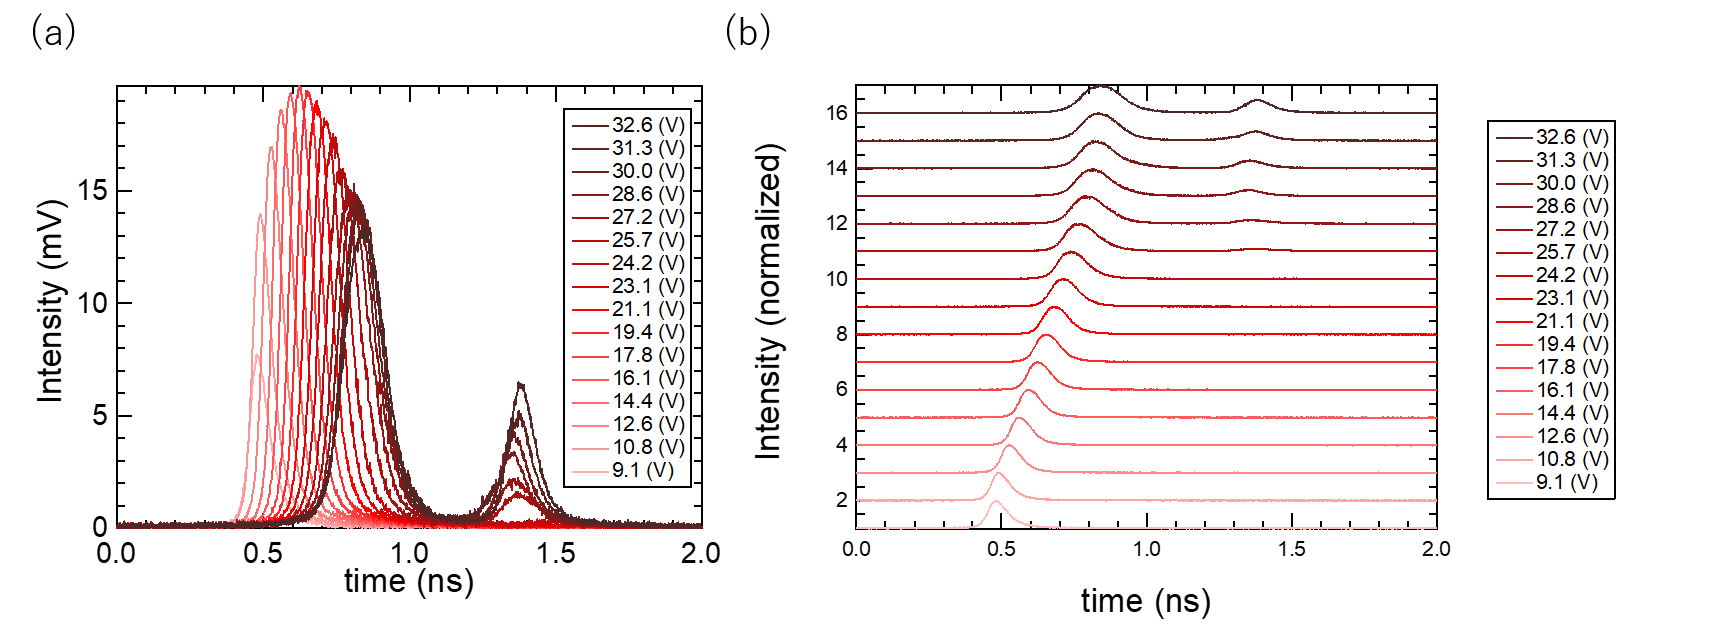
\includegraphics[width=15cm]{figure/fig_3_2_3QW_ridge_L200_GS.png}
		\caption{3MQW L=200um の利得スイッチング光パルスの時間波形}
		\label{fig:fig_3_2_3QW_ridge_L200_GS}
\end{figure}
\begin{figure}[h]
	\centering
	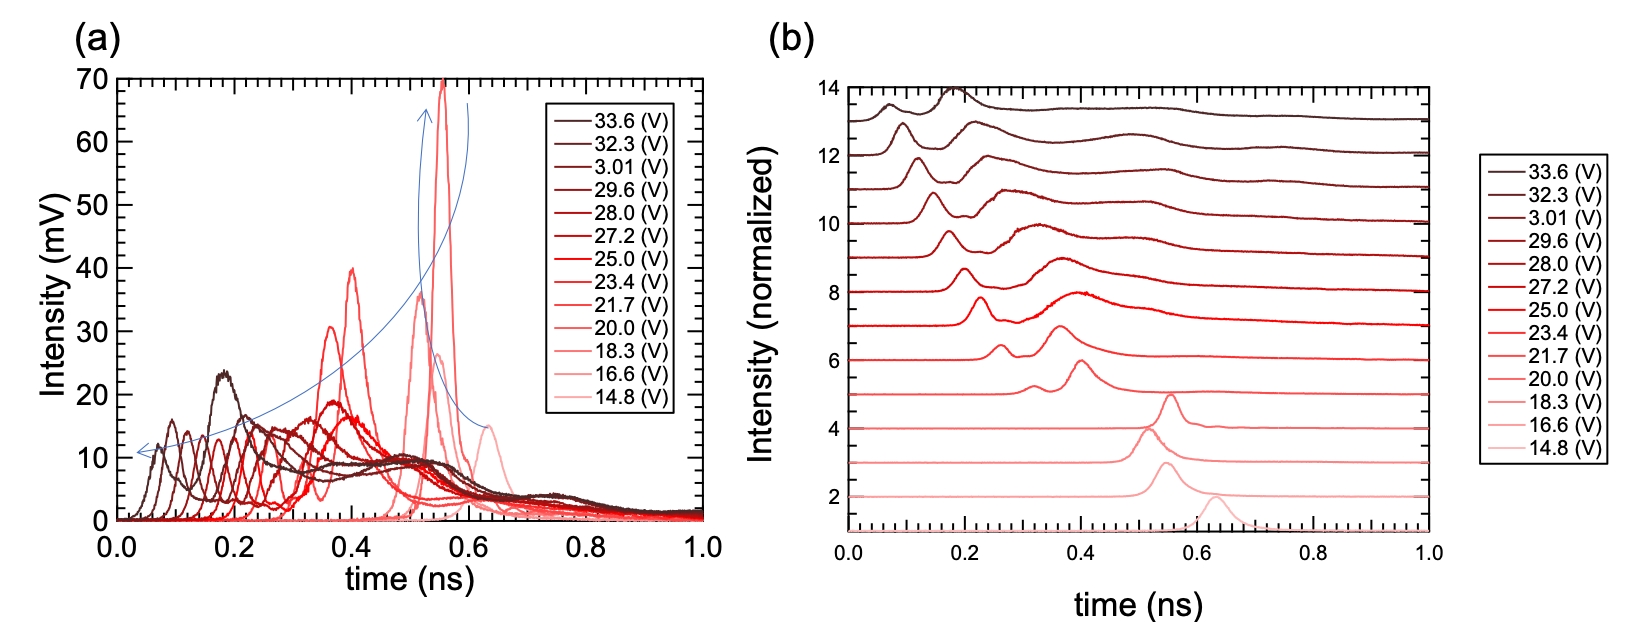
\includegraphics[width=15cm]{figure/fig_3_2_3QW_ridge_L300_GS.png}
		\caption{3MQW L=300um の利得スイッチング光パルスの時間波形}
		\label{fig:fig_3_2_3QW_ridge_L300_GS}
\end{figure}
\newpage
\clearpage
\subsection{10QW試料の利得スイッチング動作}%==============================
L=300,400,500
\begin{figure}[h]
	\centering
	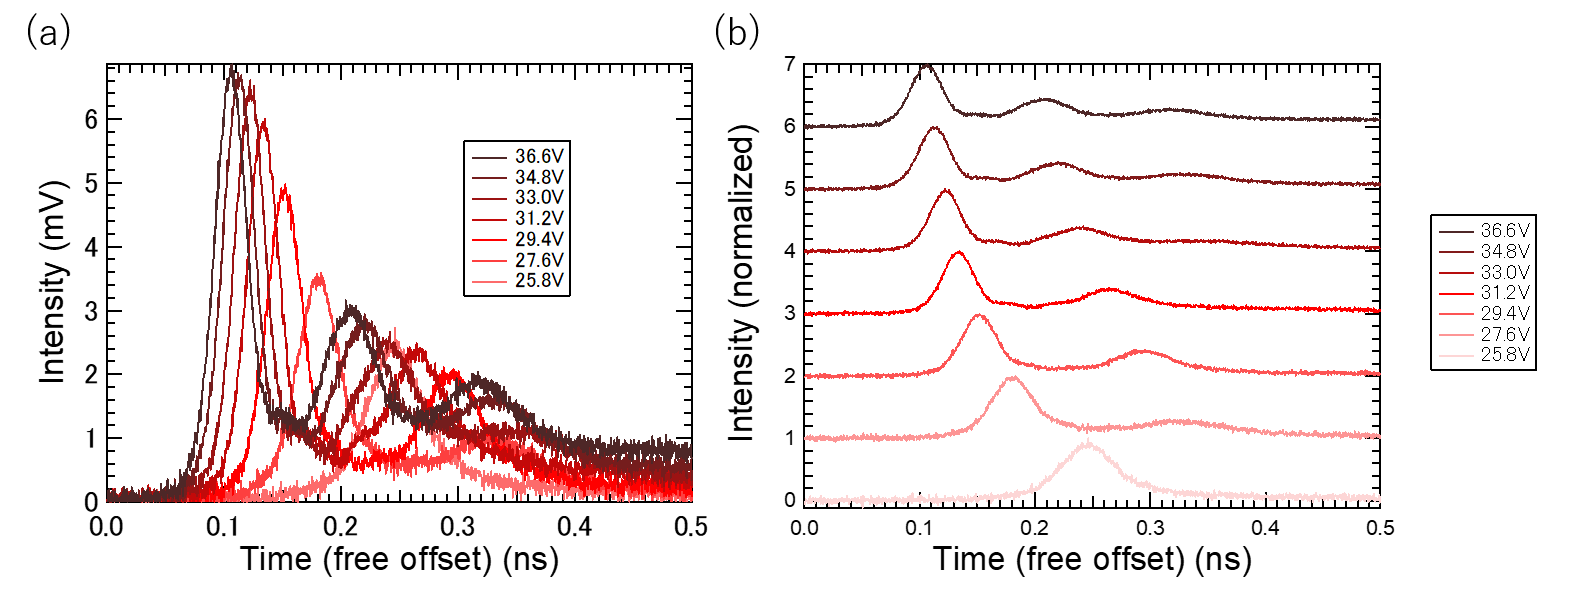
\includegraphics[width=15cm]{figure/fig_3_2_10QW_ridge_L300_GS.png}
		\caption{10MQW L=300um の利得スイッチング光パルスの時間波形}
		\label{fig:fig_3_2_10QW_ridge_L300_GS}
\end{figure}

\begin{figure}[h]
	\centering
	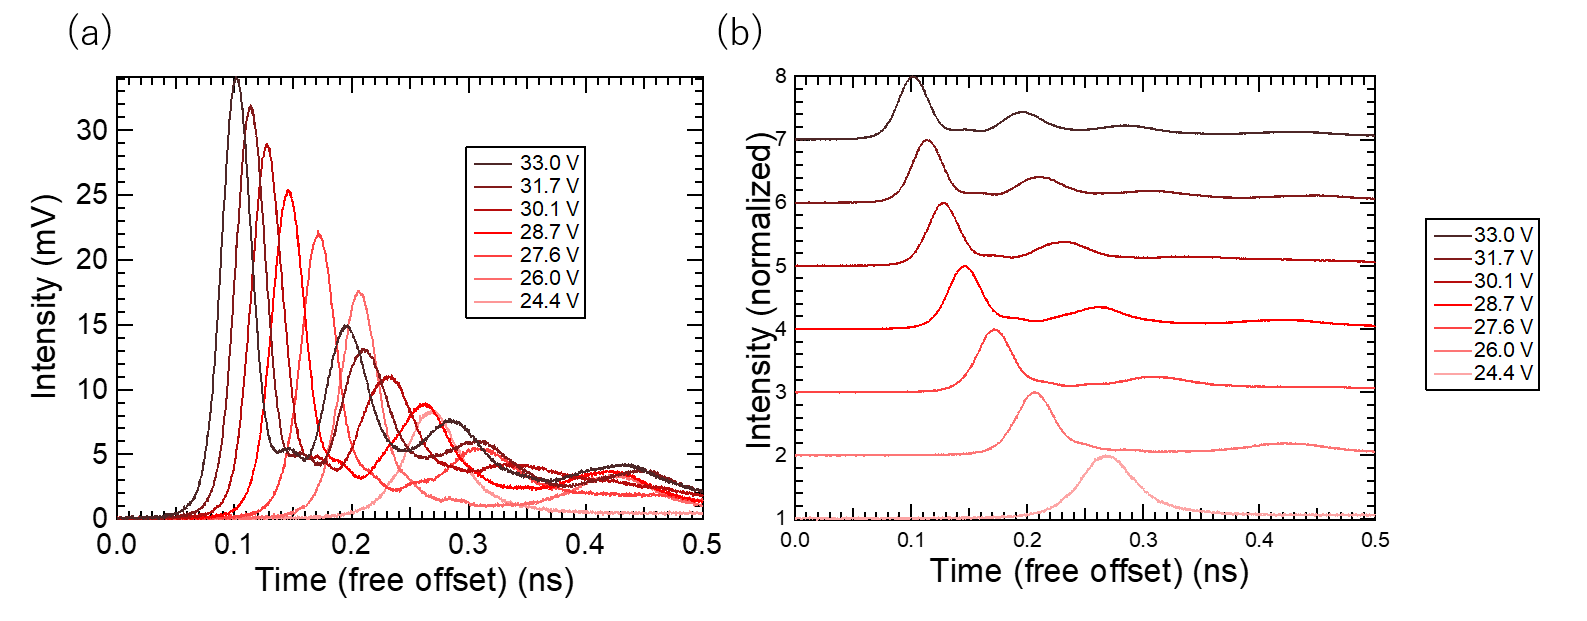
\includegraphics[width=15cm]{figure/fig_3_2_10QW_ridge_L400_GS.png}
		\caption{10MQW L=400um の利得スイッチング光パルスの時間波形}
		\label{fig:fig_3_2_10QW_ridge_L400_GS}
\end{figure}
\begin{figure}[h]
	\centering
	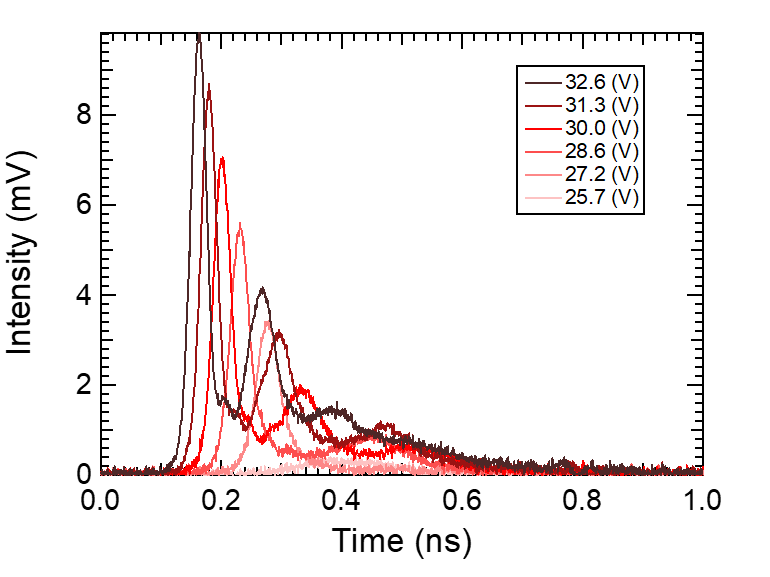
\includegraphics[width=15cm]{figure/fig_3_2_10QW_ridge_L500_GS.png}
		\caption{10MQW L=500um の利得スイッチング光パルスの時間波形}
		\label{fig:fig_3_2_10QW_ridge_L500_GS}
\end{figure}
\clearpage
\subsection{結果の比較}%===========================
FWHM をまとめた。でコンボリューション後の値を示した。
\begin{figure}[h]
	\centering
	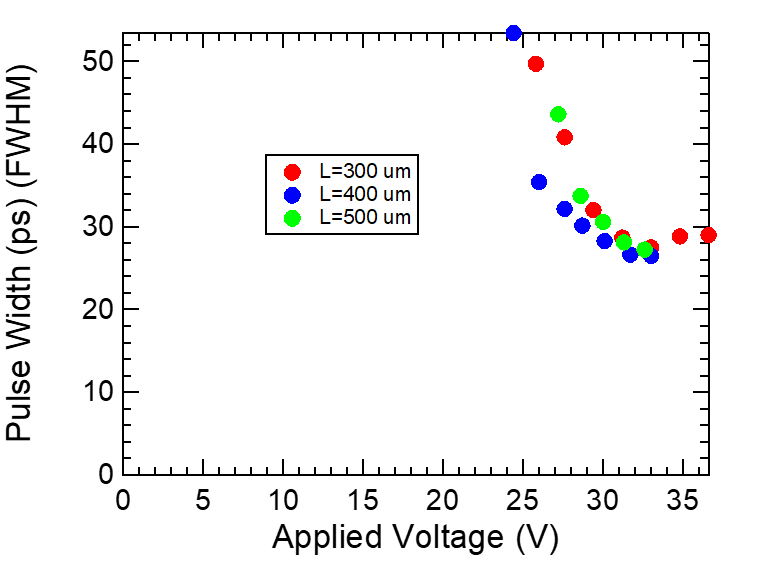
\includegraphics[width=10cm]{figure/fig_3_2_10QW_ridge_GS_FWHM.png}
		\caption{10MQW 利得スイッチングパルスのパルス幅}
		\label{fig:fig_3_2_10QW_ridge_GS_FWHM}
\end{figure}

\begin{figure}[h]
	\centering
	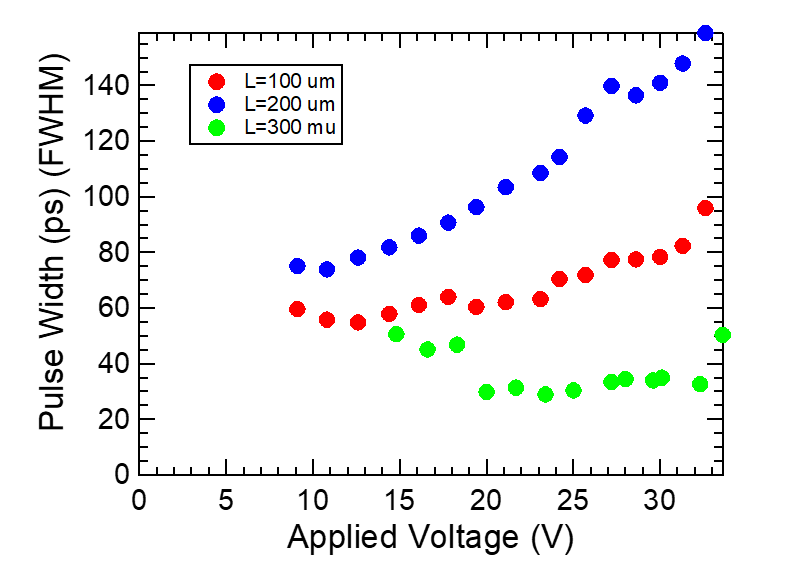
\includegraphics[width=10cm]{figure/fig_3_2_3QW_ridge_GS_FWHM.png}
		\caption{3MQW 利得スイッチングパルスのパルス幅}
		\label{fig:fig_3_2_3QW_ridge_GS_FWHM}
\end{figure}
\clearpage 
\subsection{付録かな??コンボリュージョンの説明,電気パルスの確認}%==============
\begin{comment}
\begin{figure}[h]
	\centering
	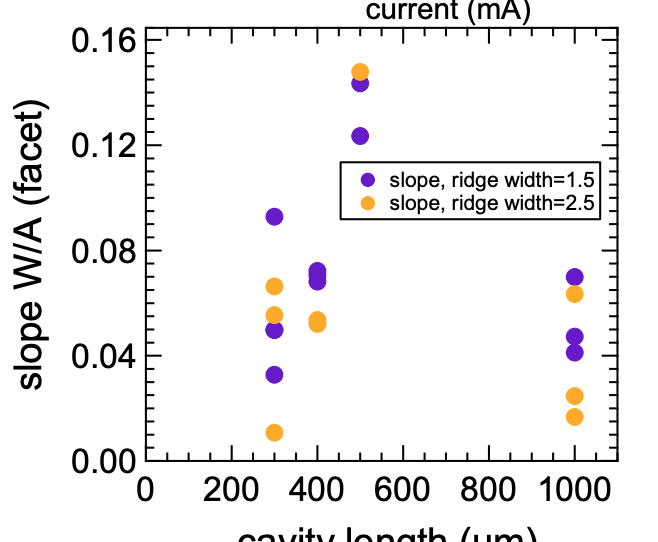
\includegraphics[width=10cm]{figure/fig_3_1_broad_slope_10QW.png}
		\caption{10MQWのスロープ}
		\label{fig_3_1_IL_broad_slope}
\end{figure}

\begin{figure}[h]
	\centering
	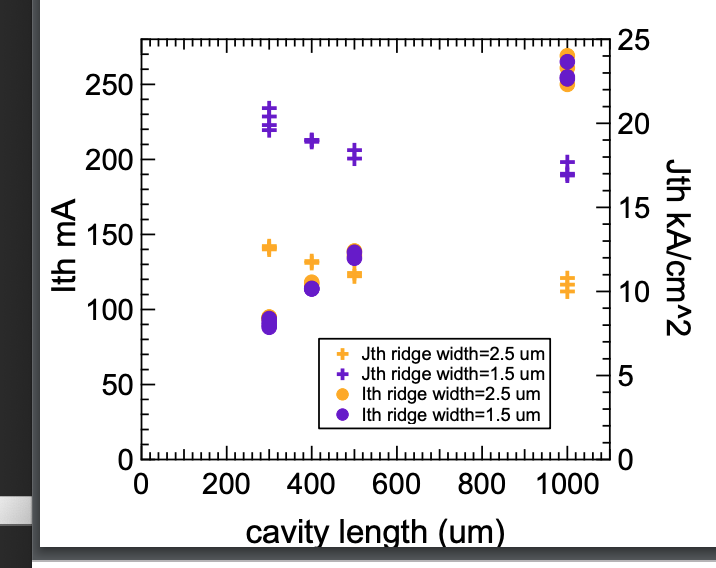
\includegraphics[width=10cm]{figure/fig_3_1_broad_i_th_10QW.png}
		\caption{10MQWの閾値電流}
		\label{fig_3_1_broad_i_th_3QW}
\end{figure}


\begin{figure}[h]
	\centering
	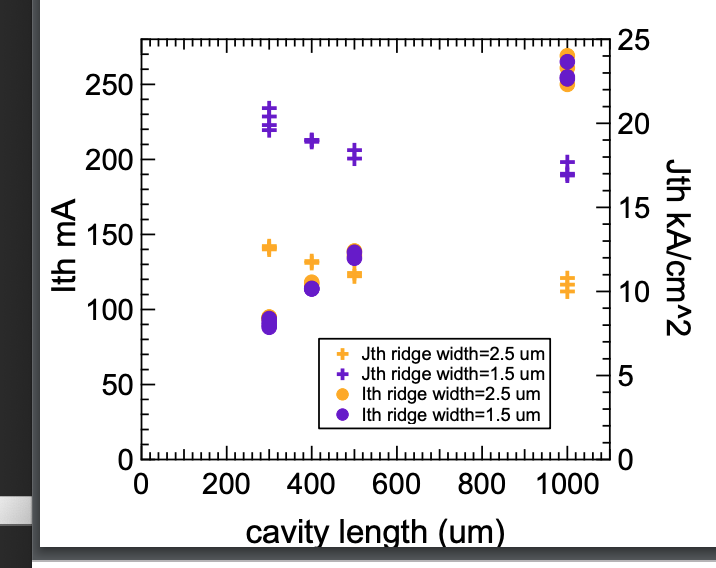
\includegraphics[width=10cm]{figure/fig_3_1_broad_i_th_10QW.png}
		\caption{10MQWの閾値電流密度のパッド幅依存性}
		\label{fig_3_1_broad_j_th_10QW}
\end{figure}
\end{comment}
